\chapter{Production Patterns and Challenges}\label{ch:production}

Building multi-agent orchestration systems for production environments introduces complexities absent from prototyping and research phases. This chapter examines the architectural patterns, operational constraints, and quality mechanisms that transform exploratory agents into reliable, scalable production systems. We focus on five critical pillars: rate limiting and token budgets, the gatekeeper pattern for API governance, retry and circuit-breaker resilience, observability and structured logging, and cost optimization strategies.

\section{Rate Limiting and Token Budgets}

Token budgets represent a fundamental constraint in production LLM-driven systems. Unlike research prototypes that consume tokens freely, production deployments must enforce spending limits per agent, per task, and per entire orchestration run. CrewAI and LangChain both provide configuration hooks for rate limiting, but the responsibility for enforcement lies in the application layer \cite{CrewAI2024}.

A token budget enforcement mechanism allocates tokens across the crew's agents proportionally to their complexity. The budget formula distributes available tokens according to agent priority and historical consumption:

\begin{equation}
B_i = B_{\mathrm{total}} \cdot \frac{w_i}{\sum_{j=1}^{N} w_j}
\label{eq:token_budget}
\end{equation}

where \(B_i\) is the budget for agent \(i\), \(B_{\mathrm{total}}\) is the total available tokens, \(w_i\) is the weight (priority or historical cost factor) for agent \(i\), and \(N\) is the number of agents. Weights are configured in JSON, never hardcoded.

Rate limiting operates at multiple layers:

\begin{enumerate}
\item \textbf{Per-Agent Limits}: Each CrewAI agent declares a maximum token budget in \texttt{agents.json}.
\item \textbf{Per-Task Limits}: Each task specifies input/output token expectations.
\item \textbf{Global Circuit Breaker}: If cumulative spend exceeds \(B_{\mathrm{total}}\), the orchestration halts and logs the overage.
\item \textbf{Provider Rate Limits}: Anthropic, OpenAI, and other providers enforce server-side rate limits; the application must respect backoff headers.
\end{enumerate}

In production, these limits prevent runaway costs and enable predictable budgeting. The gatekeeper pattern (Section \ref{sec:gatekeeper}) enforces these limits by intercepting all LLM calls.

\section{Gatekeeper Pattern}\label{sec:gatekeeper}

The gatekeeper is a single-responsibility class that mediates all external API calls—LLM inference, web search, LaTeX compilation, and file I/O. By centralizing access control, the gatekeeper enforces rate limits, logs every interaction, and provides a single point for mocking in tests \cite{Segal2026}.

The gatekeeper pattern is formalized as a decorator or wrapper around LLM provider calls. In LangChain and CrewAI, the gatekeeper wraps the LLM instance or intercepts tool invocations. Key responsibilities:

\begin{itemize}
\item \textbf{Token Accounting}: Track input and output tokens per call, sum against per-agent and global budgets.
\item \textbf{Rate Limit Enforcement}: Reject or queue calls that would exceed configured limits.
\item \textbf{Audit Logging}: Record caller, timestamp, tokens, cost, and result status.
\item \textbf{Error Handling}: Catch and classify transient vs.\ permanent failures.
\item \textbf{Metric Collection}: Export latency, throughput, and cost data for observability.
\end{itemize}

The gatekeeper does not make business decisions; it is purely administrative. This separation of concerns ensures that business logic (agent prompts, task definitions) remains isolated from infrastructure concerns (budgets, retries, logging).

\section{Retry and Circuit Breaker}

Transient failures are inevitable in distributed systems. Network timeouts, rate limit responses (HTTP 429), and temporary service outages are not logic errors; they are operational realities. The retry and circuit-breaker patterns address these gracefully \cite{LangChain2024a}.

A retry strategy specifies:

\begin{equation}
\text{Pr}[\text{retry } k] = \begin{cases} 1 & \text{if } k < K_{\max} \text{ and } f(\text{error}) \in \mathcal{T} \\ 0 & \text{otherwise} \end{cases}
\label{eq:retry_probability}
\end{equation}

where \(K_{\max}\) is the maximum number of retries, \(\mathcal{T}\) is the set of transient error codes (429, 500, 502, 503, timeout), and \(f(\text{error})\) classifies the failure. The delay between retries typically follows exponential backoff: \(\Delta_k = \Delta_0 \cdot b^k\) with jitter to avoid thundering herd problems, where \(\Delta_0\) is the initial delay (e.g., 1 second), \(b\) is the backoff multiplier (e.g., 2), and \(k\) is the retry attempt number.

A circuit breaker wraps the retry logic. If failures accumulate faster than successes over a sliding window, the circuit opens: calls fail fast without attempting the underlying operation. This prevents cascading failures and gives the downstream service time to recover. The circuit breaker has three states:

\begin{enumerate}
\item \textbf{Closed}: Normal operation; calls proceed normally. On failure, increment failure counter.
\item \textbf{Open}: Too many failures detected; calls fail immediately with a \texttt{CircuitBreakerOpen} exception. A timer resets after a threshold duration (e.g., 60 seconds).
\item \textbf{Half-Open}: Experimental state after the timer expires. A single call is allowed; if it succeeds, close the circuit. If it fails, reopen and reset the timer.
\end{enumerate}

In CrewAI and LangChain, these patterns are implemented via middleware or custom tool wrappers. The gatekeeper encapsulates both retry and circuit-breaker logic, providing a unified resilience interface.

\section{Observability and Logging}

Production systems must be observable: engineers must understand what the system is doing, why it made each decision, and where performance bottlenecks exist. Observability comprises three pillars: metrics (quantitative), logging (detailed records), and tracing (request-scoped causality).

A structured logging approach captures every significant event: agent initialization, task start/completion, LLM call details (prompt tokens, completion tokens, cost), tool invocation, error conditions, and final crew outcome. Each log entry is a JSON object with standard fields:

\begin{equation}
\text{LogEntry} = \left\{ \text{timestamp}, \text{level}, \text{logger}, \text{message}, \text{context} \right\}
\label{eq:log_entry}
\end{equation}

where \texttt{context} is a nested object carrying structured data (agent name, task ID, tokens consumed, latency milliseconds, etc.). Structured logs enable machine-readable filtering and aggregation; unstructured prose logs do not.

Observability in CrewAI and LangChain is achieved via:

\begin{itemize}
\item \textbf{Callback Hooks}: Both frameworks provide callbacks that fire on agent/task/tool events. Register a callback that emits structured logs.
\item \textbf{LLM Tracing}: LangChain LangSmith and CrewAI Telemetry export traces to external platforms.
\item \textbf{Custom Handlers}: Extend logging.Handler (Python standard library) to route JSON logs to files, cloud services, or monitoring dashboards.
\end{itemize}

In production, logs flow to a centralized store (cloud logging, ELK stack, or similar). Operators set up alerts on error rates, latency percentiles, and cost anomalies.

\begin{figure}[H]
  \centering
  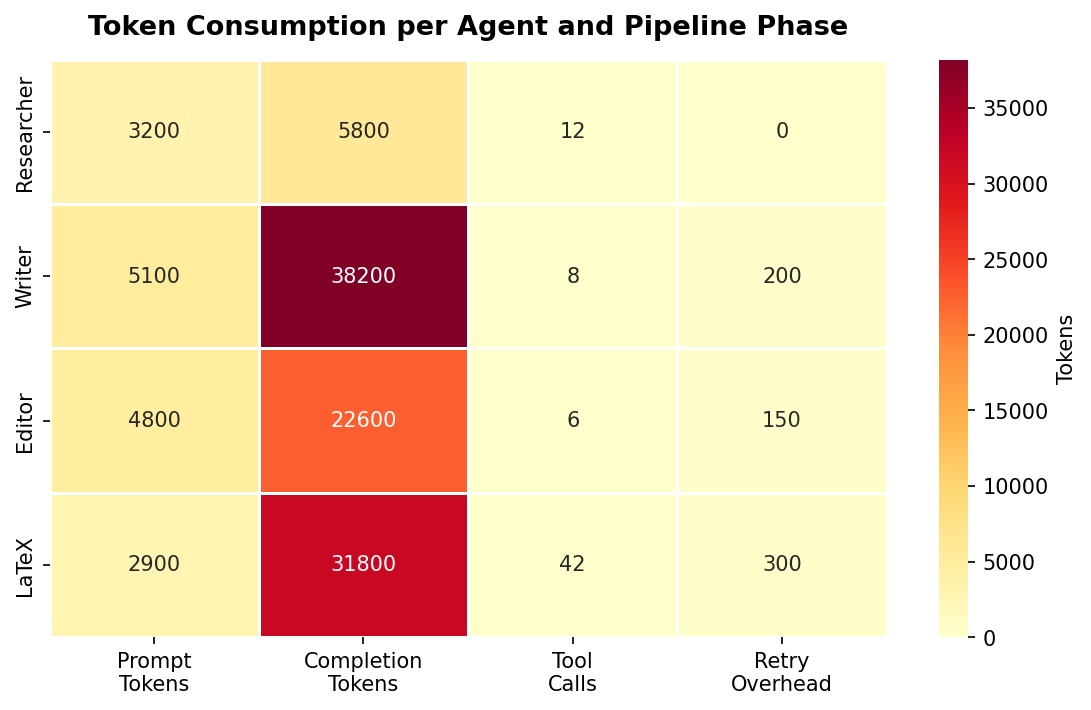
\includegraphics[width=0.88\textwidth]{figures/token_heatmap.png}
  \caption{Token consumption heatmap across agents and task phases. Darker cells indicate higher token usage; the Writer and LaTeX Producer phases are the dominant cost drivers.}
  \label{fig:token_heatmap}
\end{figure}

\section{Cost Optimization}

LLM inference is a variable operational cost. Model choice, prompt length, and call frequency all drive spending. A production system must optimize cost without sacrificing quality.

Cost accrues from two sources: input tokens (the prompt) and output tokens (the completion). Different models have different pricing; longer prompts and completions consume more tokens. The cumulative cost for a crew run is:

\begin{equation}
C = \sum_{k=1}^{K} \bigl( c_{\mathrm{in}} \cdot t_k^{\mathrm{in}} + c_{\mathrm{out}} \cdot t_k^{\mathrm{out}} \bigr)
\label{eq:cost_model}
\end{equation}

where \(K\) is the total number of LLM calls, \(c_{\mathrm{in}}\) and \(c_{\mathrm{out}}\) are the per-token prices for input and output respectively, and \(t_k^{\mathrm{in}}\) and \(t_k^{\mathrm{out}}\) are tokens for the \(k\)-th call.

Optimization strategies include:

\begin{itemize}
\item \textbf{Model Selection}: Use cheaper models (e.g., Claude Haiku) for lightweight tasks; reserve expensive models (Claude Opus) for complex reasoning \cite{Anthropic2024b}.
\item \textbf{Prompt Caching}: If the same context appears in multiple calls, cache it at the API level to reduce input token cost.
\item \textbf{Batch Processing}: Process multiple independent tasks in parallel to amortize fixed overhead.
\item \textbf{Output Constraints}: Limit output length where quality permits; use max\_tokens or early-stopping directives.
\end{itemize}

CrewAI allows per-agent LLM configuration; different agents can use different models. LangChain's LCEL enables conditional routing: invoke a cheap model first, escalate to an expensive model only if the cheap result fails quality checks. These optimization techniques are configured in JSON, not hardcoded, so operators can tune costs without code changes.

The interplay between CrewAI, LangChain, and LangGraph deserves mention here \cite{LangGraph2024}. In production, many teams deploy CrewAI for rapid prototyping, then migrate to LangGraph when state management and checkpointing become critical. LangChain serves as the lower-level abstraction layer underlying both. Understanding all three frameworks allows architects to select the right tool for each phase of the product lifecycle: exploration with CrewAI, hardening with LangGraph, and integration via LangChain \cite{CrewAI2024}, \cite{LangChain2024a}.